\subsection{Bootloaders}

\begin{frame}{GRUB}
  \begin{columns}
    \column{0.65\textwidth}
    \begin{itemize}
    \item {\em Grand Unified Bootloader}, from the GNU project
    \item De-facto standard in most Linux distributions for x86
      platforms
    \item Can read many filesystem formats to load the kernel image,
      modules and configuration
    \item Provides a menu and powerful shell with various commands
    \item Can load kernel images over the network
    \item Supports x86 legacy and UEFI systems,
      also ARM, ARM64, RISC-V, PowerPC, but less popular
      than other bootloaders on those platforms
    \item \url{https://www.gnu.org/software/grub/}
    \item \url{https://en.wikipedia.org/wiki/GNU_GRUB}
    \end{itemize}
    \column{0.35\textwidth}
    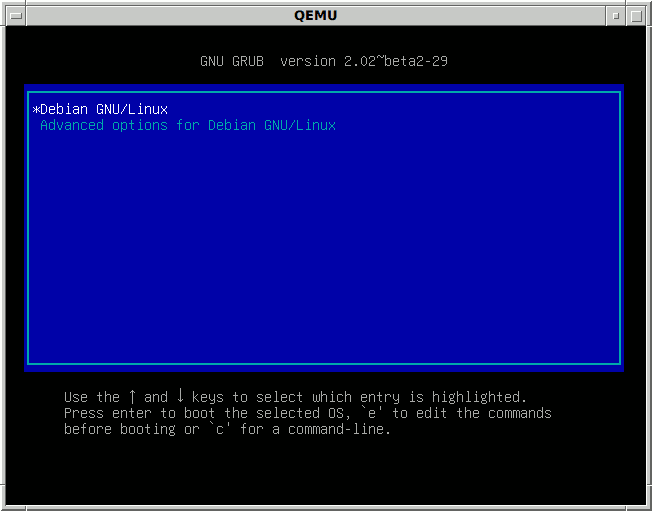
\includegraphics[width=\textwidth]{slides/linux-bootloaders-sw/grub2.png}
  \end{columns}
\end{frame}

\begin{frame}{Syslinux}
  \begin{columns}
    \column{0.8\textwidth}
    \begin{itemize}
    \item For network and removable media booting (USB key, SD card, CD-ROM)
    \item \code{syslinux}: booting from FAT filesystem
    \item \code{pxelinux}: booting from the network
    \item \code{isolinux}: booting from CD-ROM
    \item \code{extlinux}: booting from numerous filesystem types
    \item A bit rustic to build and configure, not very actively
      maintained, but still useful for specific use-cases
    \item \url{https://wiki.syslinux.org/}
    \item \url{https://kernel.org/pub/linux/utils/boot/syslinux/}
    \end{itemize}
    \column{0.2\textwidth}
    
\includegraphics[width=\textwidth]{slides/linux-bootloaders-sw/syslinux.png}
  \end{columns}
\end{frame}

\begin{frame}{systemd-boot}
  \begin{columns}
    \column{0.7\textwidth}
    \begin{itemize}
    \item Simple UEFI boot manager
    \item Useful alternative to GRUB for UEFI systems: simpler than GRUB
    \item Configured using files stored in the {\em EFI System
        Partition}
    \item Part of the {\em systemd} project, even though obviously
      distinct from {\em systemd} itself
      \begin{itemize}
      \item See our slides later in this course for more details on {\em
          systemd}
      \end{itemize}
    \item \url{https://www.freedesktop.org/wiki/Software/systemd/systemd-boot/}
    \end{itemize}
    \column{0.3\textwidth}
    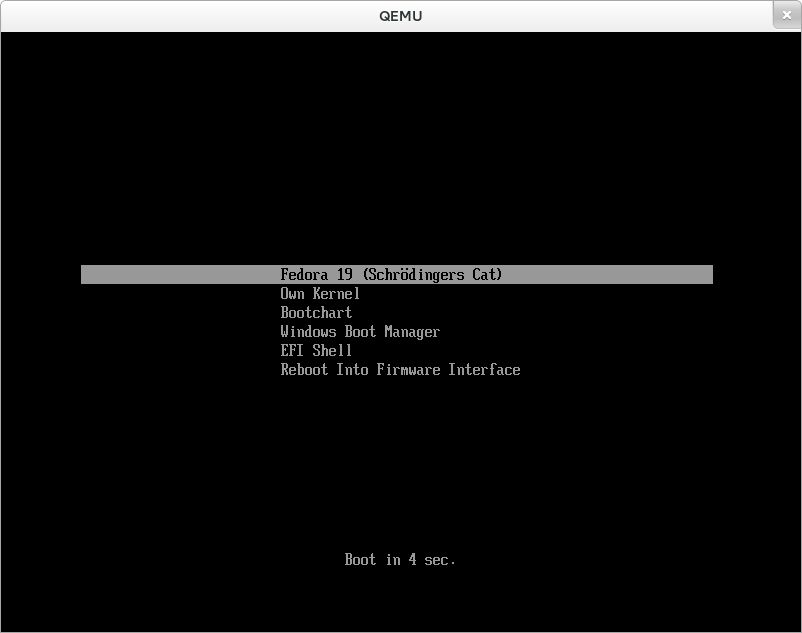
\includegraphics[width=\textwidth]{slides/linux-bootloaders-sw/systemd-boot.png}
  \end{columns}
\end{frame}

\begin{frame}{shim}
  \begin{itemize}
  \item Minimal UEFI bootloader
  \item Mainly used in secure boot scenario: it is signed by Microsoft
    and therefore successfully verified by UEFI firmware in the field
  \item Allows to chainload another bootloader (GRUB) or directly
    the Linux kernel, with signature checking
  \item \url{https://github.com/rhboot/shim}
  \end{itemize}
\end{frame}

\begin{frame}{U-Boot}
  \begin{columns}
    \column{0.7\textwidth}
    \begin{itemize}
    \item The de-facto standard and most widely used bootloader on
      embedded architectures: ARM, ARM64, RISC-V, PowerPC, MIPS, and
      more.
    \item Also supports x86 with UEFI firmware.
    \item Very likely the one provided by your SoC vendor, SoM vendor
      or board vendor for your hardware.
    \item We will study it in detail in the next section, and use it in
      all practical labs of this course.
    \item \url{https://www.denx.de/wiki/U-Boot}
    \end{itemize}
    \column{0.3\textwidth}
    
\includegraphics[width=\textwidth]{slides/linux-bootloaders-sw/u-boot.png}
  \end{columns}
\end{frame}

\begin{frame}{Barebox}
  \begin{columns}
    \column{0.7\textwidth}
    \begin{itemize}
    \item Another bootloader for most embedded CPU architectures:
      ARM/ARM64, MIPS, PowerPC, RISC-V, x86, etc.
    \item Initially developed as an alternative to U-Boot to address
      some U-Boot shortcomings
      \begin{itemize}
      \item {\em kconfig} for the configuration like the Linux kernel
      \item well-defined {\em device model} internally
      \item More Linux-style shell interface
      \item Cleaner code base
      \end{itemize}
    \item Actively maintained and developed, but
      \begin{itemize}
      \item Less widely used than U-Boot
      \item Less platform support than in U-Boot
      \end{itemize}
    \item \url{https://www.barebox.org/}
    \item Talk {\em barebox Bells and Whistles}, by Ahmad Fatoum, ELCE
      2020, \href{https://youtu.be/Oj7lKbFtyM0}{video} and
      \href{https://elinux.org/images/9/9d/Barebox-bells-n-whistles.pdf}{slides}
    \end{itemize}
    \column{0.3\textwidth}
    
\includegraphics[width=\textwidth]{slides/linux-bootloaders-sw/barebox.png}
  \end{columns}
\end{frame}
